We propose that the software be deployable into a server based virtual network running on a single system. Our hardware recommendation to run a balanced selection of elements is a quad core 16GB system with two 1TB SSD drives. The system diagram can be seen in Figure \ref{fig:deployment}.
\begin{figure*}[ht]\centering % Using \begin{figure*} makes the figure take up the entire width of the page
	\includegraphics{deployment}
	\caption{Proposed deployment of the software within the VMs on a single hardware system.}
	\label{fig:deployment}
\end{figure*}
\section{Networking layer}
\subsection{Proxmox}
Proxmox open source server virtualisation allows the deployment of several virtual machines within a hardware system. Each of these VMs can have a different balance of performance, ease of use, and security. The VMs are given only the access they need to perform the task which they are specialised for. This improves overall security. Resilience is improved since elements of the cluster can be shutdown, reinstanced, and upgraded, without impacting the whole. Snapshots and backups are simplified.
\subsection{VyOS firewall}
VyOS firewall is a Proxmox aware threat management gateway and firewall which allows more nuanced interfacing with corporate systems, while maximising the security of the VM network which sits behind it i the virtual cluster.
\subsection{Privacy aspects and using TOR etc}
Currently some compromises with privacy may be necessary. Power users vs standard users. KYC/AML. 
\href{https://bitnodes.io/nodes/?q=.onion}{tor nodes}
\section{Bitcoin value management stack}
\subsection{Bitcoin Core on NixOS}
In March 2021 \href{https://www.whitesourcesoftware.com/whitesource-npm-threat-report-for-javascript-package-registry/}{several npm packages} were compromised globally as part of the cyber warfare component of the Ruso-Ukraine war. Some components of open source Bitcoin nodes such as Thunderhub and BOS were thought to be compromised by these attacks, in that their upstream dependencies brought the vulnerabilities into the nodes. This kind of attack/vulnerability is exactly why we chose to use \href{https://github.com/fort-nix/nix-bitcoin/#features}{Nix-Bitcoin} for the most important elements of the software we are deploying for SMEs.\par
This text from the features list on github explains the enhanced security of this approach.
\begin{itemize}
\item Simplicity: Only services enabled in configuration.nix and their dependencies are installed, support for doas (sudo alternative), code is continuously reviewed and refined.
\item Integrity: The Nix package manager guarantees that all dependencies are exactly specified, packages can be built from source to reduce reliance on binary caches, nix-bitcoin merge commits are signed, all commits are approved by multiple nix-bitcoin developers, upstream packages are cryptographically verified where possible, we use this software ourselves.
\item Principle of Least Privilege: Services operate with least privileges; they each have their own user and are restricted further with systemd features, RPC whitelisting and netns-isolation. There's a non-root user operator to interact with the various services.
\item Defense-in-depth: nix-bitcoin supports a hardened kernel, services are confined through discretionary access control, Linux namespaces, dbus firewall and seccomp-bpf with continuous improvements.
\end{itemize}
\subsection{LDK based Sensei}
\href{https://l2.technology/sensei}{Sensei} is a new node implementation which uses a hub and spoke model to allow light nodes to operate lightning channels without running the whole Bitcoin stack themselves. This is potentially useful for the client side of the deployment.
\subsection{Object and media tracking: nostr}
The world database in the shared rooms in the metaverse is the global object master, with nostr and perhaps another technology tracking these objects.\par
\section{Addressing identified risks}
\chapter{Current example deployment }
\begin{figure*}[ht]\centering % Using \begin{figure*} makes the figure take up the entire width of the page
	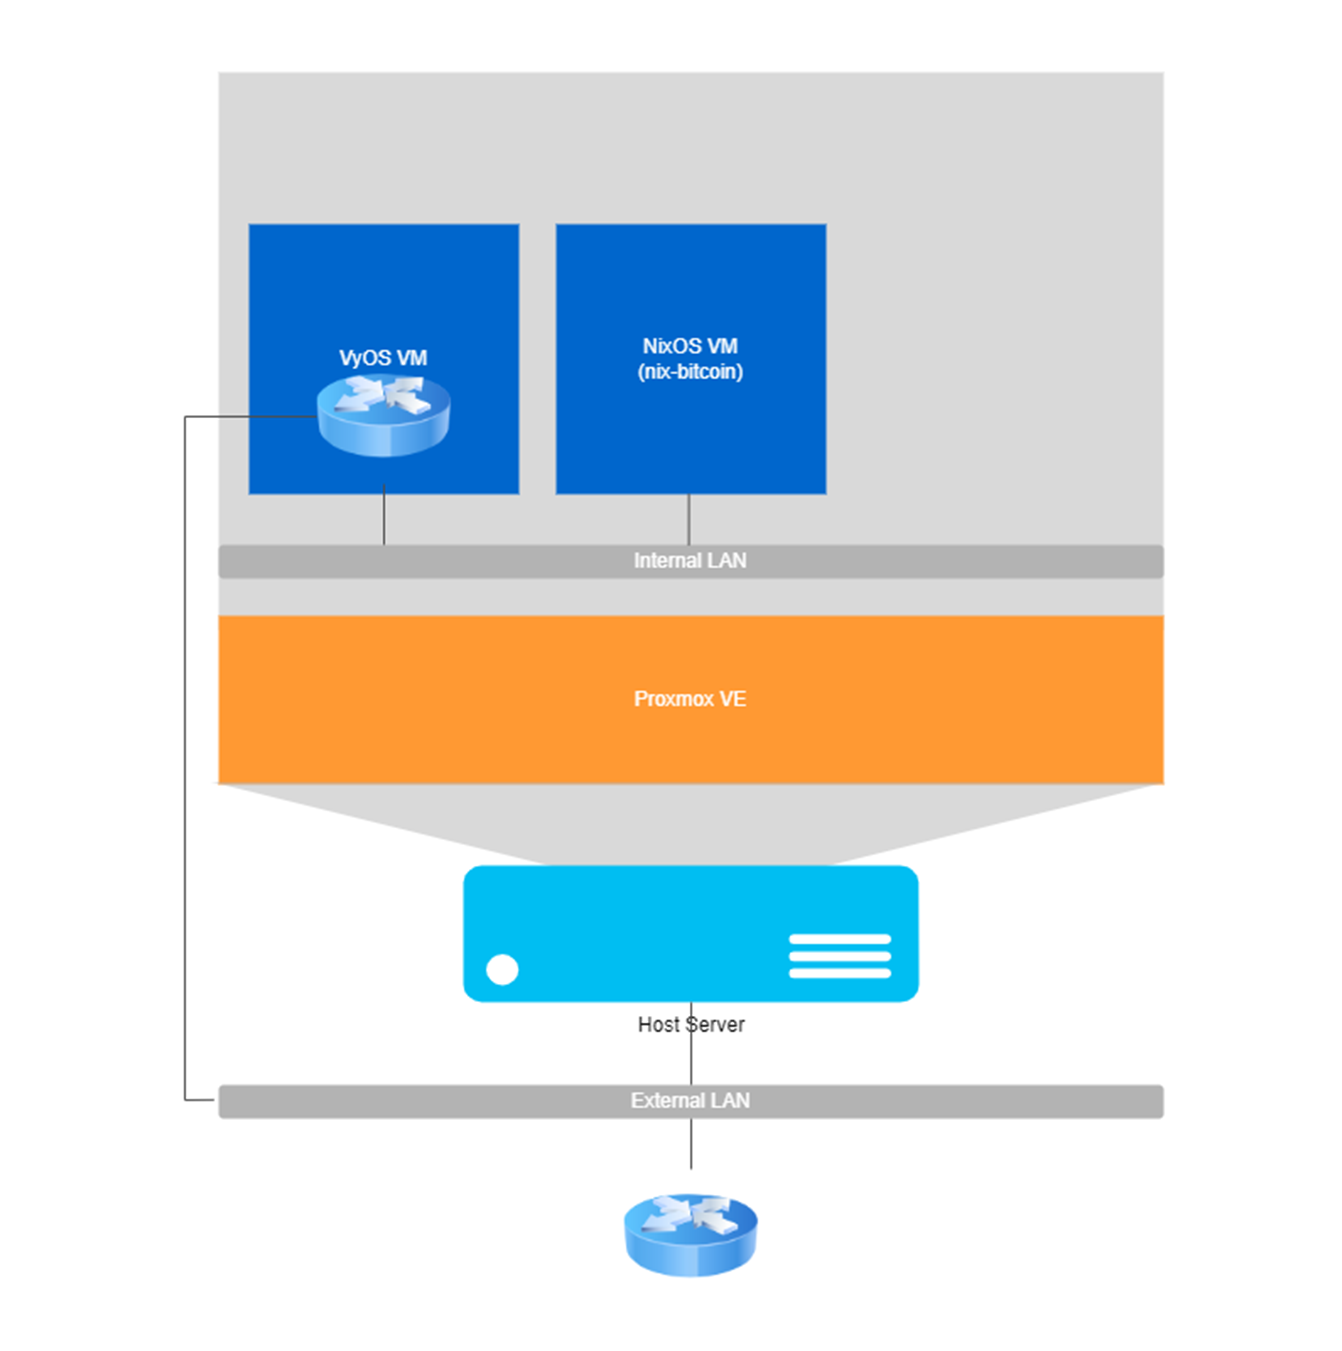
\includegraphics{proxmoxmap}
	\caption{Current diagram of the proxmox as seen on the github.}
	\label{fig:proxmoxmap}
\end{figure*}
\section{GitHub }
